\section{Introduction}
\label{intro}
Images are the most rich source of multimedia data on the Web.
Present keyword-based search technology and information extraction
techniques enable effective image search by keywords.
For example, if one enters the keyword ``kiwi'' on Google Image search engine
we got a whole screen of images which are associated with the term ``kiwi'',
according to Google (see \figref{fig:search-kiwi-on-google}).
However, the term ``kiwi'' refers to at least two different entities:
{\em kiwi the bird} and {\em kiwi the fruit}. Google apparently doesn't
distinguish between these two entities and it mixes their images together.
The ranking of these images is probably determined by the relevance
ranking of the web pages that contain these images.
Like Google, most other image search engine also return a mixed list of images
without classifying the results by their different senses.
Ambiguous entities like ``kiwi'' are abundant in real-world. For example,
there are at least three different entities for ``Polo'',
four for ``Andrew Appel'', six for ``Anderson'' and over
ten for ``Lei Zhang'' on Google Image.

\begin{figure}[h]
\begin{center}
\centering
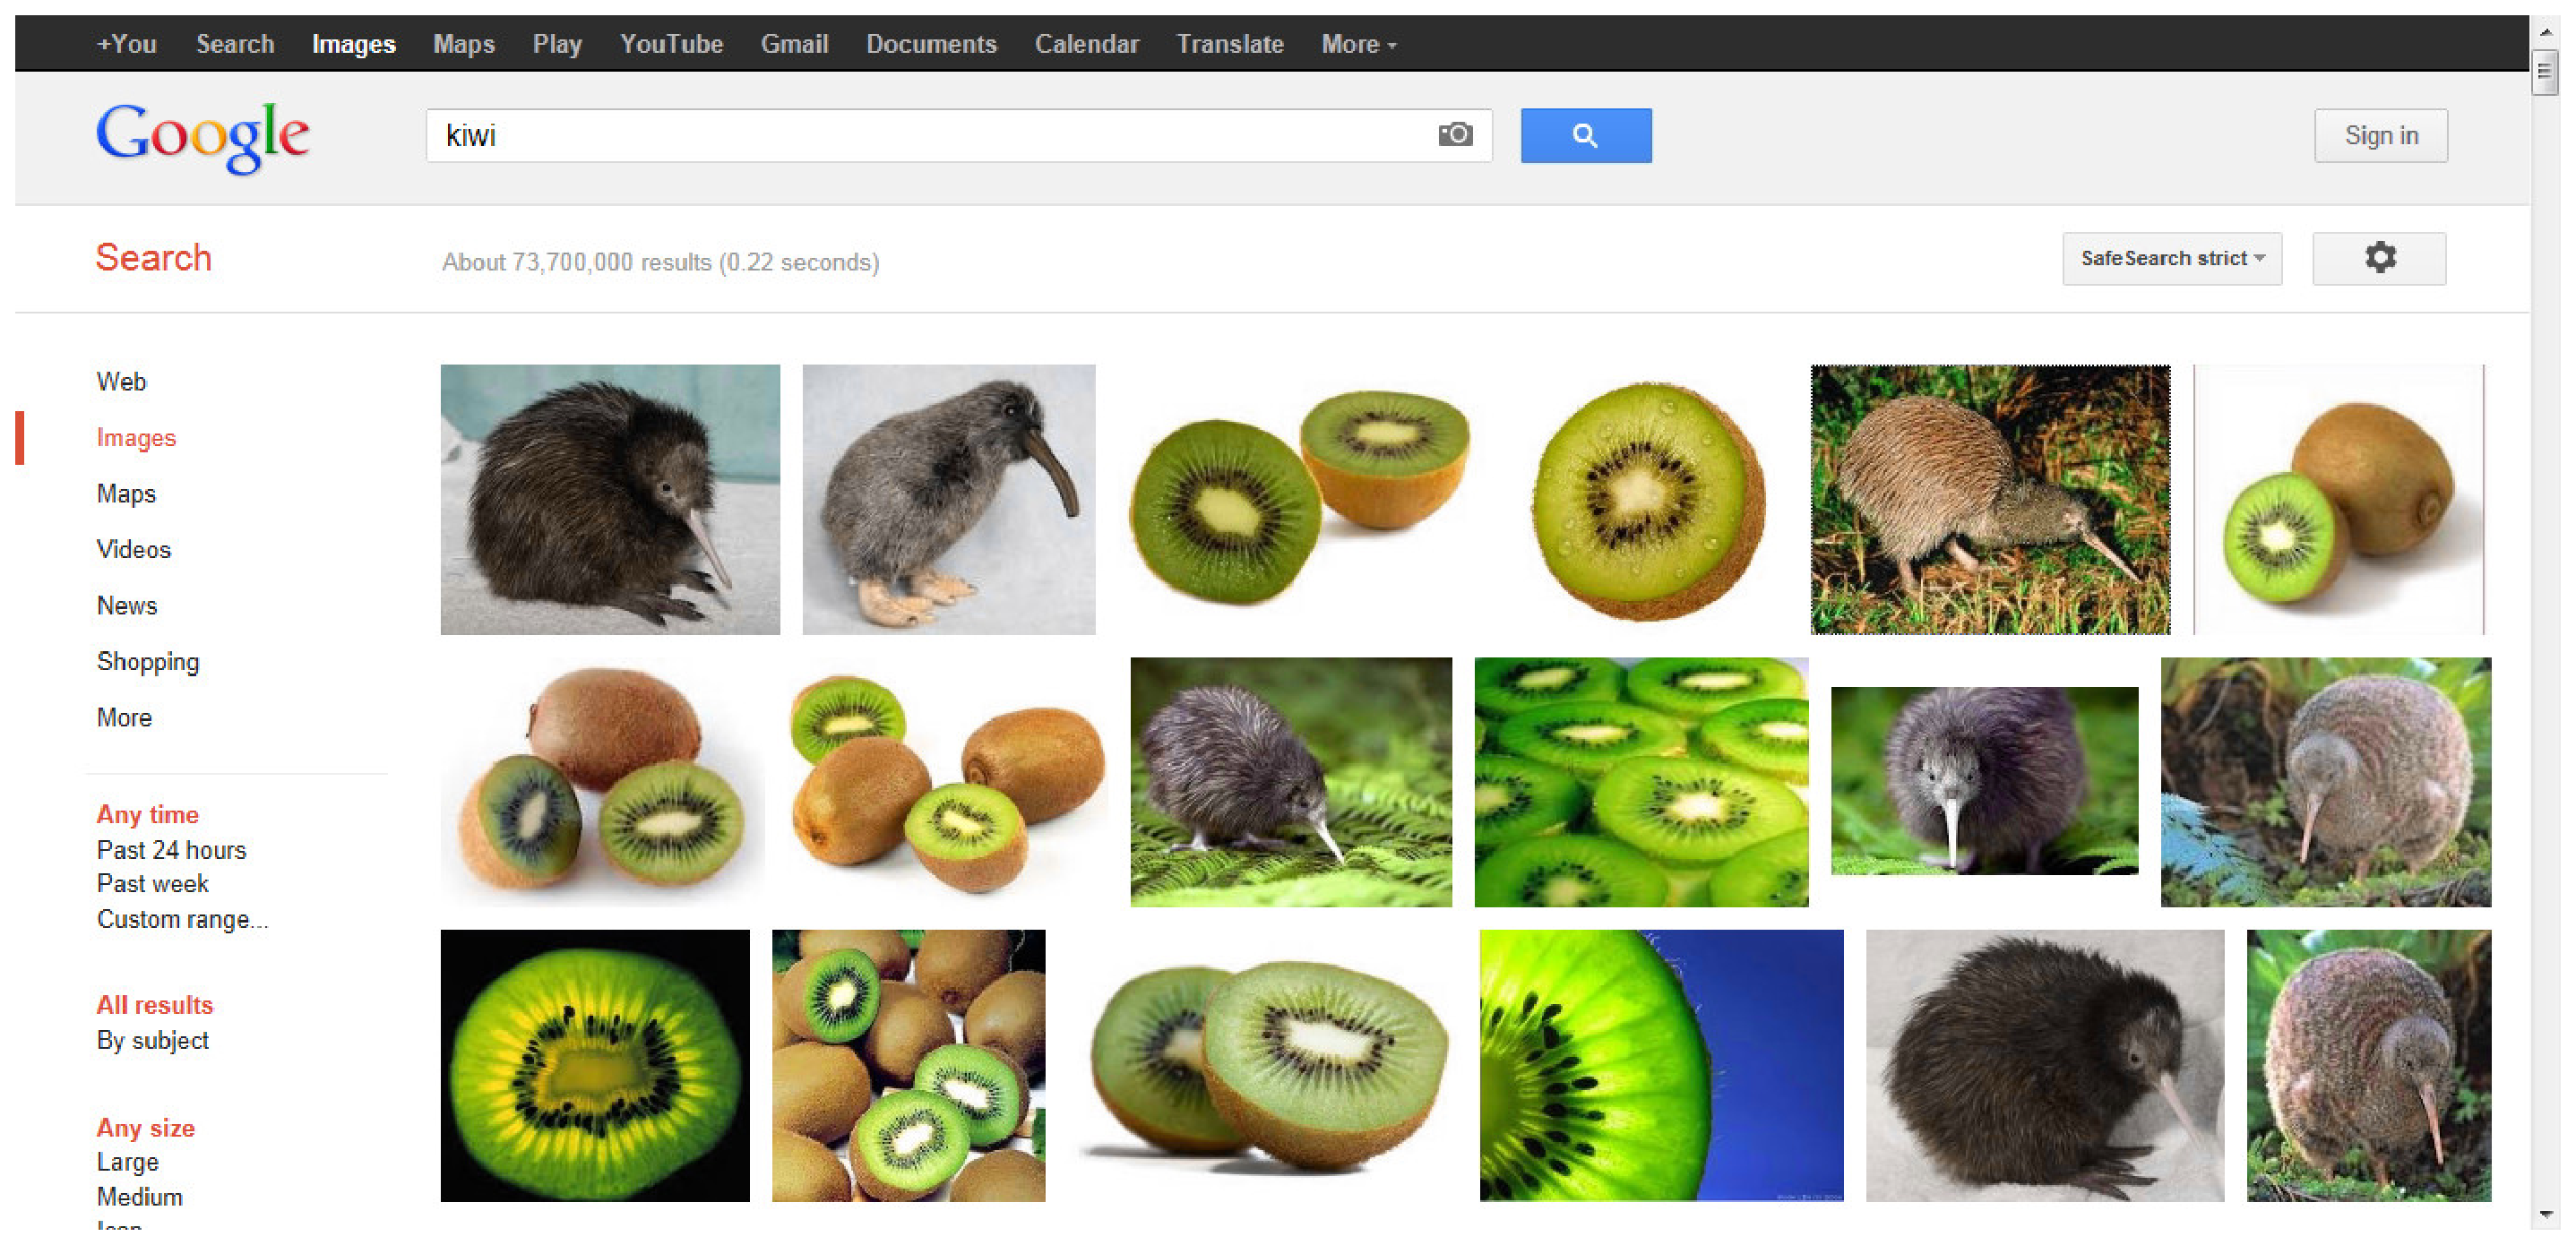
\includegraphics[width=0.9\columnwidth]{search_kiwi.eps}
\caption{Search result of keyword ``kiwi'' on Google Image}
\label{fig:search-kiwi-on-google}
\end{center}
\end{figure}

But when a user search for the term ``kiwi'', it is quite likely that he's
looking for either the bird or the fruit but not both. Having to scroll through
pages of images to locate the images that he wants is not a very good
user experience. A better search result interface would be to divide the
result window into sections, where each section contains only a number of
images of the same type of entities. User can then pick a section of interest
and expand it further to see more images of that entity.

%It will be more convenient for the users to distinguish from the
%result get what they desire if we divided the result into individual clusters further.
%All images belong to these two sorts of entity are mixed and disorderly placed as the search engine
%doesn't know what's in the image on earth. But for the user requesting for ``kiwi'',
%he must be interested in a single entity sharing this keyword such as the kiwi bird.
%At this moment all kiwi fruit images are useless because what he want is the
%bird. He has to through over all the result and filter out the unwanted items
%manually.
% {\it Apple is not a extremly example here because it is easy to distinguish any ``apple'' from two.
% Some other cases to show this?}

This paper is concerned with the problem of clustering a set of
images indexed by the same keyword on an image search engine into
multiple groups, each of which containing a distinct entity.

There are three existing approaches to image clustering. The first is
``content-based'' approach which uses only visual signals from
the images themselves \cite{ZhongLL11}.
Most content-based image clustering 
%can be either unsupervised or semi-supervised. Unsupervised 
approaches extract low-level visual features such as color and basic shapes
from the images and use these to construct feature vector for similarity
comparison. 
%Semi-supervised approach usually leverages visual object
%recognition and uses the object annotations for clustering. 
The problem with these approaches is that web images about the same entity
can be very diverse and low level visual cues are often inadequate to
capture the semantic commonality among the images. Take the images of
the kiwi birds in \figref{fig:search-kiwi-on-google} for example,
the background, color, pattern, brightness, contrast and
orientation of the images can be quite different from image to image.
An alteration of the above approach leverages visual object 
recognition and uses the object annotations for clustering.
However, it cannot succeed in our problem because
object recognition requires supervised learning and works only for a limited
types of objects which have been manually labeled. Even for those
manually trained object recognition tasks, the
state-of-the-art techniques \cite{Li09scene} still suffers from
low accuracy.

The second is ``context-based'' approach which uses only the surrounding
text, URL or tags of the images as feature space \cite{Cai2004b}. %\cite{Cai2004}
The challenge here is
1) finding the right context and 2) modeling the context. Existing
techniques use visual cues from the web page to segment the page into
blocks and uses the block that contains the image as its context. To model
the context, all previous work uses variants of bag of words model which
has limited capability of capturing the semantics of the text.

The third is a hybrid approach which combines visual features with textual
features \cite{Fu2011}.
Because of the different nature in these two feature sources,
there's no easy way of creating a combined / uniform signal for an image
or using one single similarity function in the clustering.
As such, existing methods often adopts a two-phase
approach, taking advantage of the visual signals in one phrase, and the
text signals in another. However, on many occasions, visual feature
similarity and textual similarity of the context can conflict with each other
so the above two-phrase approach can be counter-productive.
%For instance, the image in \figref{fig:kiwibird} appears to be a bird
%though the surrounding text talks about kiwi the fruit.
%This example also shows that
%visual method alone cannot classify web images correctly.

%\begin{figure}[th]
%\centering
%%\includegraphics[width=0.6\columnwidth]{kiwi_example.eps}
%\epsfig{file=kiwi_example.eps, width=0.3\columnwidth}
%\caption{A kiwi bird that looks also like a fruit}
%\label{fig:kiwibird}
%\end{figure}

%Most previous work on image search results clustering
%\cite{Chang1984,Smith1996,ZhongLL11,Fu2011}
%focuses on clustering visual signals from the image content and then
%complementing them with signals from the surrounding text of the images.
%There are two challenges faced by these algorithms.
%First, there is a semantic disconnect
%between the visual signals and the text signals. While these algorithms can
%extract low-level visual features such as color and shapes from the images,
%and can also extract words and phrases from the surrounding text,
%it is difficult to combine these two information sources to create
%comprehensive semantics of the image.
%Second, most existing methods treats the text
%
%The mainly problem of these algorithms is the gap between visual
%and textual information. These algorithms could extract some low-level
%visual signal of the images, but it's
%not so easy to obtain the textual signals from the visual ones. This is the
%``semantic gap''.
%
%There are some novel image search results clustering algorithms which
%made use of textual information of the images.
%%\cite{Cai2004b,Cai2004,Feng2004,Gao2005,Jing2006}
%They extract some textual signals to obtain semantic information, some of these
%researches even use both visual and textual information and then combine them.
%The most popular textual signals are surrounding texts, URLs, image descriptions
%and so on.

%Cai et al. made some progress in their paper \cite{Cai2004b,Cai2004}.
%He represent a method to reduce the gap between
%visual and text information, use a page segmentation algorithm named VIPS to
%extract text information, which is mentioned in \cite{VIPS}. They gave three
%kinds of representations for images: visual feature based representation,
%textual feature based representation and link graph based representation. Since
%they think this it's an open problem for extracting sematic information by
%visual feature of pictures, they only use textual feature and link graph to
%finish their two-level clustering algorithm.

%Li et al. \cite{LiXLMZ05} introduced a novel method to process
%inhomogeneous information. With this method, we can select different clustering
%algorithm for each feature, then merge them into a global loss function.
%They use simple bag-of-word method to deal with textual information, and use
%their algorithm to combine that with low-level features. The performance
%(micro-average precision) is much better than concatenating low level features
%and word frequency vector to a ``long'' vector and clustering with k-means.
%
%Fu et al. \cite{Fu2011} applied a constraint propagation framework for
%multi-modal situations. The existing constraint propagation algorithm can only be
%used in the the scenario of single-modal, that is either for text feature or for
%visual feature. Fu use constraint graph model to represent each modal and use random
%walk to pass the constraints between the graphs.
%
%All the above researches were just using the plain
%surrounding text, and they didn't move forward any step to process the plain
%text. It's somehow insufficient, because traditional bag-of-word method could
%not exactly show the meaning of a passage, especially when the
%passage is short.
%

In this paper, we present a prototype system that takes the context-base
clustering to the next level. We take this approach because 1) there are
two possibly conflicting sources of signals for a given image:
the visual signal and the text signal and there is no simple way to combine
or reconcile them; and 2) text signals are more reliable and can be better
captured by our novel techniques. In our framework,
we extract two types of context of a given image: the HTML <IMG> tag context
which consist of the URL and ALT name of the image,
and the surrounding plain text context. We then conceptualize these context
into a list of weighted Wikipedia concepts and cluster the images
based on these concepts.
%
%with a refined sibling
%algorithm, and then perform a \textit{Conceptualization} method on these text.
%Then we could get a concept vector for each concept, which will contain much
%more semantic information than the word itself. In order to make good use of the
%signals of an image, we classify the text features into two categories. One is
%\textit{Inner features} which is the features from the image itself, including URL and image
%title. The other is \textit{Outer features} such as surrounding context.
%
We adopt a tri-stage
clustering algorithm to obtain image clusters with high accuracy.

This paper hence makes three main contributions:
1) We developed a method to extract and conceptualize the image context
using an external knowledge source;
2) Our novel tri-stage clustering algorithm yields clusters on
benchmark web images with high accuracy;
3) The prototype system also characterises each cluster with a
ranked list of concepts.
%One is we use external knowledge base to support text feature based clustering.
%Since the context of an image maybe very short,
%knowledge base driven approach can help merge some images with very
%little amount of contexts. The other is our approach can
%conceptualize each cluster to a set of weighted concepts which
%can indicate the meaning of the cluster.
%
%Although we have had the concept vector, it's still a difficult problem to
%cluster the search results. Since we will never know the number of clusters,
%we choose \textit{Hierarchical Agglomerative Clustering} (HAC) algorithm in
%our work. The other reason we use HAC is, as HAC holds a hierarchy structure
%of clustering, it's easy to expand it to an incremental version.

%The other question is, how to determine the similarity between the search
%results. Here we use a \textit{Vector Space Model} (VSM), and use
%\textit{Cosine Similarity} to compute pairwise similarity.
% TODO: expand this part.

%(Paragraph for IHAC)
% TODO: IHAC should be mentioned here.

% The challenges in image clustering:
% Some work have been done relative to this problem: JIA[x] YI[y] BING[z], why aren't they good enough
% Our approach:
% Our contribution:
